\documentclass{article} 
\usepackage{tikz} 
\begin{document} 
\begin{center} 
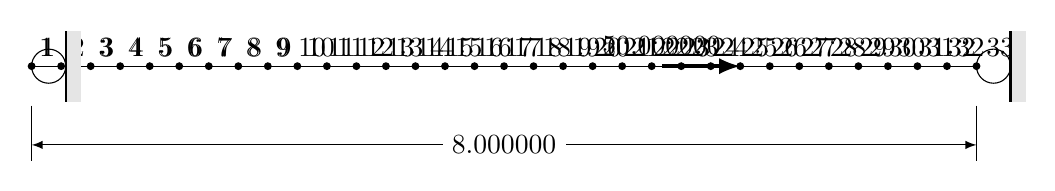
\begin{tikzpicture} 
% estilos de linea y relleno 
\tikzstyle{carga} = [ultra thick,latex-]  
% definicion apoyo de segundo genero 
% #1: ubicación del apoyo 
% #2: angulo de rotacion 
 \newcommand{\apoyoseg}[2]{ 
\coordinate (O) at #1; 
\begin{scope}[rotate around={#2:(O)}] 
\fill [black!10](O) ++(-0.45,-0.433013) rectangle ++(0.9,-0.2); 
\draw [thick] (O) ++(-0.45,-0.433013) -- ++(0.9,0); 
\draw (O) -- ++(-0.25,-0.433013) -- ++(0.45,0) -- cycle; 
\end{scope} 
 } 
% definicion apoyo de primer genero 
% #1: ubicación del apoyo 
% #2: angulo de rotacion 
 \newcommand{\apoyopri}[2]{ 
\coordinate (O) at #1; 
\begin{scope}[rotate around={#2:(O)}] 
\fill [black!10](O) ++(-0.45,-0.433013) rectangle ++(0.9,-0.2); 
\draw [thick] (O) ++(-0.45,-0.433013) -- ++(0.9,0); 
\draw (O) ++(0,-0.216506) circle (0.216506); 
\end{scope} 
 } 
% definicion carga puntual 
% #1: ubicación de la carga 
% #2: rótulo de la carga 
% #3=1: carga positiva, #3=-1: carga negativa 
% #4=1,#5=0: carga en x, #4=0,#5=1: carga en y 
% #6=0: carga entrando al nudo, #6=1: carga saliendo del nudo 
% #7: ubicación del rótulo de la carga 
\newcommand{\cargapun}[7]{ 
\path #1 ++(#6*#4,#6*#5) coordinate (O); 
\draw [carga] (O) -- ++(-1.0*#3*#4,-1.0*#3*#5) 
node [#7] {#2}; 
 } 
% cota horizontal 
% #1: coordenada punto inicial () 
% #2: coordenada punto final () 
% #3: rotulo de la cota 
% #4: separación entre puntos y cota 
% #5: separación entre puntos y inicio de marcas 
% #6: separación entre cota y fin de marcas 
\newcommand{\cotahori}[6]{ 
\path #1 ++(0,#4) coordinate (A); 
\path #2 ++(0,#4) coordinate (B); 
\draw [latex-latex] (A) -- (B) 
node [midway,fill=white] {#3}; 
\path #1 ++(0,#5) coordinate (C); 
\path #1 ++(0,#4+#6) coordinate (D); 
\draw (C) -- (D); 
\path #2 ++(0,#5) coordinate (C); 
\path #2 ++(0,#4+#6) coordinate (D); 
\draw (C) -- (D); 
 } 
% cota vertical 
% #1: coordenada punto inicial () 
% #2: coordenada punto final () 
% #3: rotulo de la cota 
% #4: separación entre puntos y cota 
% #5: separación entre puntos y inicio de marcas 
% #6: separación entre cota y fin de marcas 
\newcommand{\cotavert}[6]{ 
\path #1 ++(#4,0) coordinate (A); 
\path #2 ++(#4,0) coordinate (B); 
\draw [latex-latex] (A) -- (B) 
node [midway,fill=white] {#3}; 
\path #1 ++(#5,0) coordinate (C); 
\path #1 ++(#4+#6,0) coordinate (D); 
\draw (C) -- (D); 
\path #2 ++(#5,0) coordinate (C); 
\path #2 ++(#4+#6,0) coordinate (D); 
\draw (C) -- (D); 
 } 
% dibujar elementos 
\tikzstyle{elem}=[draw=black,thin]; 
\tikzstyle{nudo}=[midway,above]; 
\begin{scope}[elem] 
\draw (0.000000,0.000000)--(0.375000,0.000000) node[nudo] {1}; 
\draw (0.375000,0.000000)--(0.750000,0.000000) node[nudo] {2}; 
\draw (0.750000,0.000000)--(1.125000,0.000000) node[nudo] {3}; 
\draw (1.125000,0.000000)--(1.500000,0.000000) node[nudo] {4}; 
\draw (1.500000,0.000000)--(1.875000,0.000000) node[nudo] {5}; 
\draw (1.875000,0.000000)--(2.250000,0.000000) node[nudo] {6}; 
\draw (2.250000,0.000000)--(2.625000,0.000000) node[nudo] {7}; 
\draw (2.625000,0.000000)--(3.000000,0.000000) node[nudo] {8}; 
\draw (3.000000,0.000000)--(3.375000,0.000000) node[nudo] {9}; 
\draw (3.375000,0.000000)--(3.750000,0.000000) node[nudo] {10}; 
\draw (3.750000,0.000000)--(4.125000,0.000000) node[nudo] {11}; 
\draw (4.125000,0.000000)--(4.500000,0.000000) node[nudo] {12}; 
\draw (4.500000,0.000000)--(4.875000,0.000000) node[nudo] {13}; 
\draw (4.875000,0.000000)--(5.250000,0.000000) node[nudo] {14}; 
\draw (5.250000,0.000000)--(5.625000,0.000000) node[nudo] {15}; 
\draw (5.625000,0.000000)--(6.000000,0.000000) node[nudo] {16}; 
\draw (6.000000,0.000000)--(6.375000,0.000000) node[nudo] {17}; 
\draw (6.375000,0.000000)--(6.750000,0.000000) node[nudo] {18}; 
\draw (6.750000,0.000000)--(7.125000,0.000000) node[nudo] {19}; 
\draw (7.125000,0.000000)--(7.500000,0.000000) node[nudo] {20}; 
\draw (7.500000,0.000000)--(7.875000,0.000000) node[nudo] {21}; 
\draw (7.875000,0.000000)--(8.250000,0.000000) node[nudo] {22}; 
\draw (8.250000,0.000000)--(8.625000,0.000000) node[nudo] {23}; 
\draw (8.625000,0.000000)--(9.000000,0.000000) node[nudo] {24}; 
\draw (9.000000,0.000000)--(9.375000,0.000000) node[nudo] {25}; 
\draw (9.375000,0.000000)--(9.750000,0.000000) node[nudo] {26}; 
\draw (9.750000,0.000000)--(10.125000,0.000000) node[nudo] {27}; 
\draw (10.125000,0.000000)--(10.500000,0.000000) node[nudo] {28}; 
\draw (10.500000,0.000000)--(10.875000,0.000000) node[nudo] {29}; 
\draw (10.875000,0.000000)--(11.250000,0.000000) node[nudo] {30}; 
\draw (11.250000,0.000000)--(11.625000,0.000000) node[nudo] {31}; 
\draw (11.625000,0.000000)--(12.000000,0.000000) node[nudo] {32}; 
\end{scope} 
% dibujar nudos 
\tikzstyle{nudo}=[fill=black,above right]; 
\def \r{0.05}; 
\begin{scope}[nudo] 
\fill (0.000000,0.000000) circle (\r) node {1}; 
\fill (0.375000,0.000000) circle (\r) node {2}; 
\fill (0.750000,0.000000) circle (\r) node {3}; 
\fill (1.125000,0.000000) circle (\r) node {4}; 
\fill (1.500000,0.000000) circle (\r) node {5}; 
\fill (1.875000,0.000000) circle (\r) node {6}; 
\fill (2.250000,0.000000) circle (\r) node {7}; 
\fill (2.625000,0.000000) circle (\r) node {8}; 
\fill (3.000000,0.000000) circle (\r) node {9}; 
\fill (3.375000,0.000000) circle (\r) node {10}; 
\fill (3.750000,0.000000) circle (\r) node {11}; 
\fill (4.125000,0.000000) circle (\r) node {12}; 
\fill (4.500000,0.000000) circle (\r) node {13}; 
\fill (4.875000,0.000000) circle (\r) node {14}; 
\fill (5.250000,0.000000) circle (\r) node {15}; 
\fill (5.625000,0.000000) circle (\r) node {16}; 
\fill (6.000000,0.000000) circle (\r) node {17}; 
\fill (6.375000,0.000000) circle (\r) node {18}; 
\fill (6.750000,0.000000) circle (\r) node {19}; 
\fill (7.125000,0.000000) circle (\r) node {20}; 
\fill (7.500000,0.000000) circle (\r) node {21}; 
\fill (7.875000,0.000000) circle (\r) node {22}; 
\fill (8.250000,0.000000) circle (\r) node {23}; 
\fill (8.625000,0.000000) circle (\r) node {24}; 
\fill (9.000000,0.000000) circle (\r) node {25}; 
\fill (9.375000,0.000000) circle (\r) node {26}; 
\fill (9.750000,0.000000) circle (\r) node {27}; 
\fill (10.125000,0.000000) circle (\r) node {28}; 
\fill (10.500000,0.000000) circle (\r) node {29}; 
\fill (10.875000,0.000000) circle (\r) node {30}; 
\fill (11.250000,0.000000) circle (\r) node {31}; 
\fill (11.625000,0.000000) circle (\r) node {32}; 
\fill (12.000000,0.000000) circle (\r) node {33}; 
\end{scope} 
% dibujar apoyos 
\apoyopri{(0.000000,0.000000)}{90} 
\apoyopri{(12.000000,0.000000)}{90} 
% dibujar cargas puntuales 
\cargapun{(9.000000,0.000000)}{50.000000}{1.000000}{1}{0}{0}{above} 
% dibujar cotas 
\cotahori{(0.000000,0.000000)}{(12.000000,0.000000)}{8.000000}{-1}{-0.5}{-0.2} 
\end{tikzpicture} 
\end{center} 
\end{document} 
